\documentclass[12pt,a4paper]{amsart}
% ukazi za delo s slovenscino -- izberi kodiranje, ki ti ustreza
\usepackage[slovene]{babel}
%\usepackage[cp1250]{inputenc}
\usepackage[T1]{fontenc}
\usepackage[utf8]{inputenc}
\usepackage{amsmath,amssymb,amsfonts}
\usepackage{url}
\usepackage{graphicx}
%\usepackage[demo]{graphicx}
%\usepackage[normalem]{ulem}
\usepackage[dvipsnames,usenames]{color}
\usepackage{hyperref}
\hypersetup{
     colorlinks   = true,
     citecolor    = gray
}

\graphicspath{ {./slike/} }
% ne spreminjaj podatkov, ki vplivajo na obliko strani
\textwidth 15cm
\textheight 24cm
\oddsidemargin.5cm
\evensidemargin.5cm
\topmargin-5mm
\addtolength{\footskip}{10pt}
\pagestyle{plain}
\overfullrule=15pt % oznaci predlogo vrstico


% ukazi za matematicna okolja
\theoremstyle{definition} % tekst napisan pokoncno
\newtheorem{definicija}{Definicija}[section]
\newtheorem{primer}[definicija]{Primer}
\newtheorem{opomba}[definicija]{Opomba}

\renewcommand\endprimer{\hfill$\diamondsuit$}


\theoremstyle{plain} % tekst napisan posevno
\newtheorem{lema}[definicija]{Lema}
\newtheorem{izrek}[definicija]{Izrek}
\newtheorem{trditev}[definicija]{Trditev}
\newtheorem{posledica}[definicija]{Posledica}


% za stevilske mnozice uporabi naslednje simbole
\newcommand{\R}{\mathbb R}
\newcommand{\N}{\mathbb N}
\newcommand{\Z}{\mathbb Z}
\newcommand{\C}{\mathbb C}
\newcommand{\Q}{\mathbb Q}

% ukaz za slovarsko geslo
\newlength{\odstavek}
\setlength{\odstavek}{\parindent}
\newcommand{\geslo}[2]{\noindent\textbf{#1}\hspace*{3mm}\hangindent=\parindent\hangafter=1 #2}

% naslednje ukaze ustrezno popravi
\newcommand{\program}{Finančna matematika} % ime studijskega programa: Matematika/Finan"cna matematika
\newcommand{\imeavtorja}{Tina Bertok\\ Neža Habjan \\ Gašper Letnar} % ime avtorja
\newcommand{\imementorja}{prof. dr. Riste Škrekovski} % akademski naziv in ime mentorja
\newcommand{\naslovdela}{Genetski algoritem na problemu potujočega trgovca}
\newcommand{\letnica}{2018} %letnica 




\begin{document}

% od tod do povzetka ne spreminjaj nicesar
\thispagestyle{empty}
\noindent{\large
UNIVERZA V LJUBLJANI\\[1mm]
FAKULTETA ZA MATEMATIKO IN FIZIKO\\[5mm]
\program\ -- 1.~stopnja}
\vfill

\begin{center}{\large
\imeavtorja\\[2mm]
{\bf \naslovdela}\\[10mm]
Projekt v povezavi z OR\\[1cm]}

\end{center}
\vfill

\noindent{\large
Ljubljana, \letnica}
\pagebreak

\thispagestyle{empty}
\hypersetup{linkcolor = black}
\tableofcontents
\pagebreak

\section{Navodilo}

Implement the genetic algorithm metaheuristic for TSP. Present the chromosomes as ordered
lists i.e. as paths. Apply different variations for the crossover operations, such as order crossover
(OX), paritally mapped crossover (PMX), cycle crossover (CX), etc. Experiment with different
sizes of the population. You can generate some of the testing graphs yourself, and you can find
some of them on the Internet.

\newpage
\section{Uvod}

Naša naloga je, da implementiramo genetski algoritem na problemu potujočega trgovca. Pri tem bomo uporabljali različna križanja, spreminjali velikosti populacije in verjetnosti za mutacijo. Primerjali bomo rezultate pri različnih pogojih. Naš algoritem bomo testirali na podatkih, ki jih bomo generirali sami in na podatkih najdenih na internetu. 
\\
\\
\textit{Genetski algoritem} je metahevristika, navdihnjena s strani procesov naravne selekcije in spada v razred razvojnih
algoritmov. Uporablja se za generiranje kvalitetnih rešitev v optimizaciji, ki temeljijo na operatorjih kot so mutacija, križanje
in selekcija.  
\\
V genetskem algoritmu se uporabi množica kandidatov za rešitev, ki jih nato razvijamo do čim boljše rešitve. Vsak kandidat
ima določene lastnosti, katere lahko spremenimo oziroma lahko mutirajo. Evolucija rešitev se ponavadi začne na naključni izbiri kandidatov, katere potem s pomočjo iteracije razvijamo. Na vsakem iterativnem koraku se potem oceni primernost novih kandidatov za optimizacijski problem. Najboljše kandidate potem uporabimo za naslednji korak iteracije. Algoritem se zaključi, ko je izpolnjen zaustavitveni kriterij. Ena možnost je, da algoritem ustavimo po tem, ko preteče določeno število generacij.
\\
\\
\textit{Problem trgovskega potnika} oz. \textit{traveling salesman problem (TSP)} je NP-težek problem v kombinatorični optimizaciji, pomemben pri operacijskih raziskavah, matematični optimizaciji in teoretičnemu računalništvu. Trgovski potnik mora obiskati določeno množico mest tako, da bo pri tem prehodil čim krajšo pot in se vrniti v izhodišče.
\\
\\
Pri programiranju in pisanju algoritma smo se odločili za programski jezik Python, saj imamo v njem največ znanja. Pri projektu pa smo spoznali še knjižnico \textit{matplotlib} za delo z grafi. 
\\

\newpage
\section{Opis dela}
\
\subsection{Osnovne funkcije}
\
\\
\\
Že dobro poznan problem potujočega , smo se odločili predstaviti z grafom v obliki $n \times n$ matrike cen povezav. Graf smo generirali tako, da smo elemente matrike, ki predstavljajo celoštevilske cene povezav, izbrali naključno. To je prikazano v spodnji funkciji \textit{utezi(n, maxCena)}.

\begin{figure*}[ht]
\centering
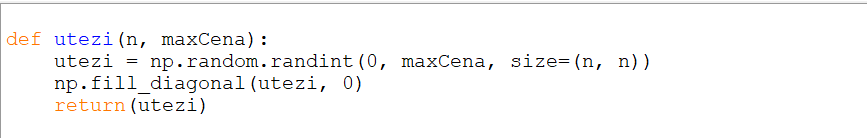
\includegraphics[width=1\textwidth]{utezi}
\end{figure*}

Nato je bilo potrebno definirati \textit{ciljno funkcijo} oz. \textit{fitness function}, s pomočjo katere bomo ocenjevali primernost rešitev. V našem primeru je vrednost te funkcije za neko pot kar dolžina te poti.

\begin{figure*}[ht]
\centering
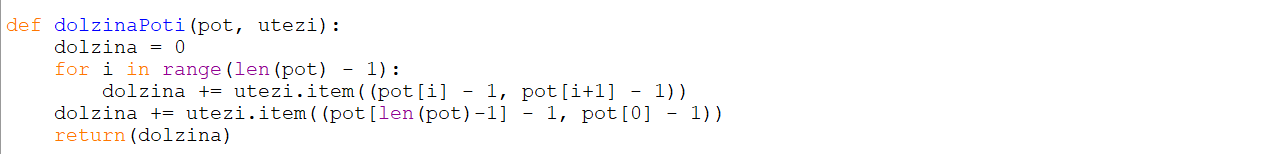
\includegraphics[width=1\textwidth]{dolzinapoti}
\end{figure*}
Naključno smo ustvarili začetno populacijo izbrane velikosti. Vsak element populacije ali \textit{kromosom} predstavlja neko pot, ki obišče vsa vozlišča grafa. 
\\

\begin{figure*}[ht]
\centering
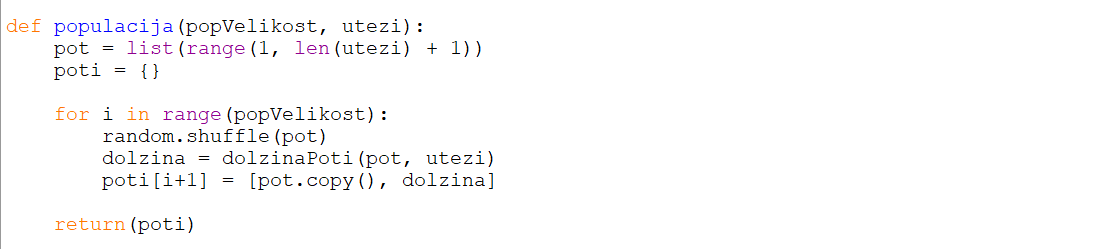
\includegraphics[width=1\textwidth]{populacija}
\end{figure*}
\newpage
V nadaljevanju izberemo starše, katerih gene bomo uporabili za nastanek naslednje generacije - določimo paritveni bazen. Tega se bomo lotili postopoma in sicer izbiramo po 2 starša za 2 otroka. Za selekcijo imamo dve možnosti, in sicer selekcijo s turnirjem ter proporcionalno selekcijo. Odločili smo se za turnirsko. Vsakega starša bomo izbrali tako, da bomo iz trenutne populacije naključno izbrali  $k$ kromosomov oz. poti. Naša funkcija oz. \textit{selekcija} nam bo vrnila zmagovalca izmed teh  $k$ poti oziroma pot z najkrajšo dolžino. Torej bomo za $n$ staršev v bazenu imeli $n$ turnirjev.

\begin{figure*}[ht]
\centering
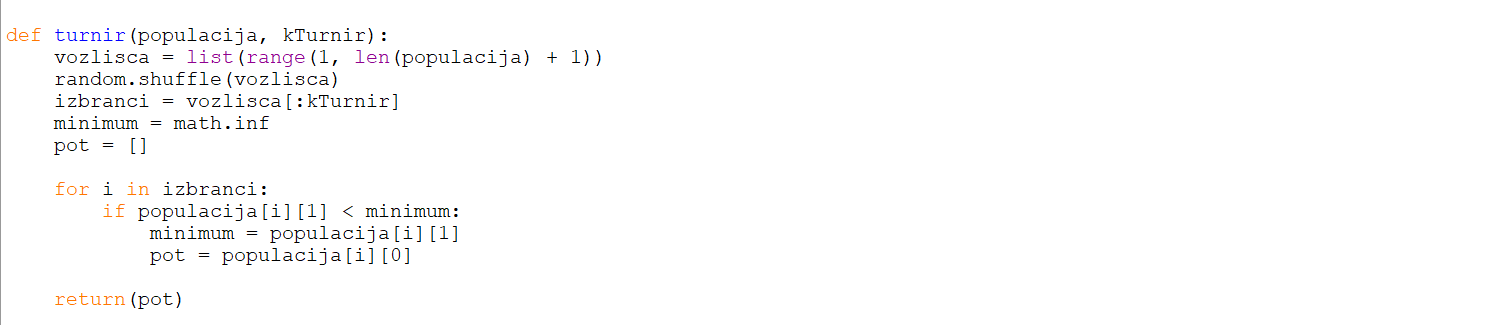
\includegraphics[width=1\textwidth]{turnir}
\end{figure*}

\subsection{Križanja oziroma crossoverji}
\
\\
\\
Za ustvarjanje otrok bomo uporabili različna križanja oz. \textit{crossoverje} staršev (poti) iz paritvenega bazena. Pri tem smo uporabili različne variacije križanj: 
\\
\subsubsection{Urejeno križanje ali ordered crossover}
\
\\
\\
V urejenem križanju ali OX vsak starš predstavlja neko zaporedje vseh vozlišč. Na začetku oba starša razdelimo na tri podzaporedja, kjer 1. podzaporedje predstavlja vozlišča od prvega do vključno tistega na a-tem mestu, 2. podzaporedje poteka od vozlišča na a-tem do vključno vozlišča na b-tem mestu, 3. podzaporedje pa predstavlja preostanek osnovnega zaporedja. Prvi potomec ima kopirano 2. podzaporedje prvega starša na enaki poziciji. Nato od b+1 mesta naprej nadaljujemo z vozlišči drugega starša, ki jih dopolnjujemo (v primeru da je to vozlišče že vsebovano v zaporedju otroka, ga preskočimo) najprej iz 3. podzaporedja, nato 1. podzaporedja in nazadnje še iz 2. podzaporedja. Ko se zaporedje konča, skočimo na začetek in postopek nadaljujemo vse do začetka a-tega mesta. 
Na enak način tvorimo drugega otroka, le da vlogi staršev zamenjamo.

\begin{figure*}[ht]
\centering
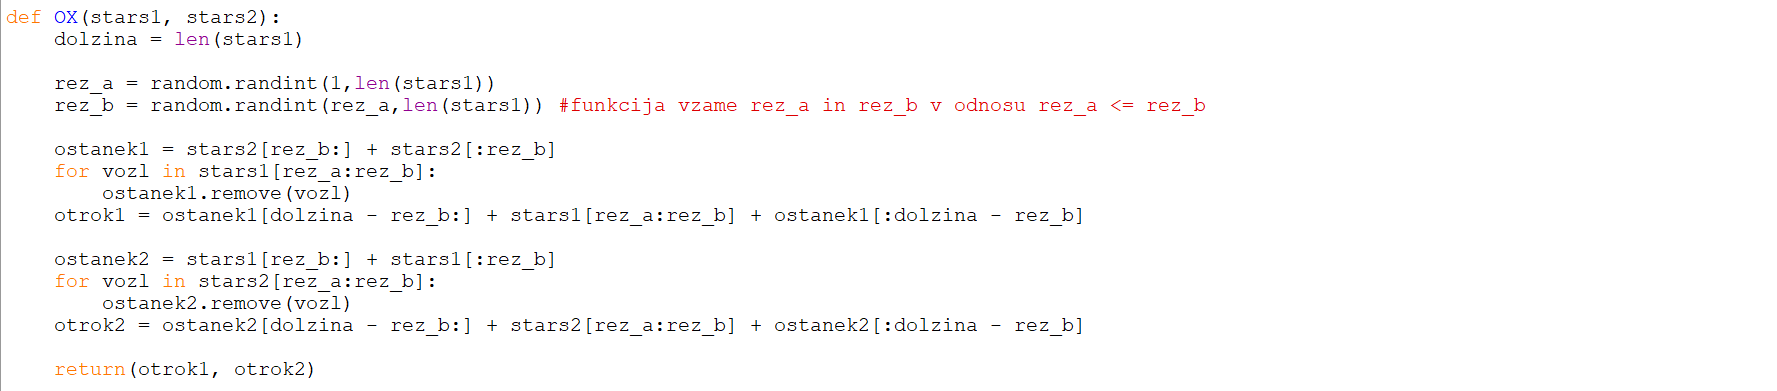
\includegraphics[width=1\textwidth]{OX}
\end{figure*}
\newpage
\subsubsection{Delno mapirano križanje ali partially mapped crossover}
\
\\
\\
Drugi način križanja je delno mapirano križanje ali PMX, v katerem starša spet razdelimo na tri podzaporedja. Prvemu otroku prav tako kot v OX, prepišemo vrednosti prvega starša med obema rezoma, se pravi 2. podzaporedje. Nato vsako vozlišče(vsaka vrednost i) iz 2. podzaporedja drugega starša, ki še ni vsebovano v zaporedju otroka, dobi svoj istoležeči par v prvem staršu. Če je ta par že vsebovan v 2. podzaporedju drugega starša, temu vozlišču ponovno poiščemo par iz prvega starša in to počnemo dokler dobljeni istoležeči par v drugem staršu ne leži izven 2. podzaporedja.  Takrat na njegovo mesto (v drugem staršu) zapišemo vrednost i. Na koncu postopka vsa prazna mesta v otroku zapolnimo z istoležečimi vozlišči iz drugega starša. 

\begin{figure*}[ht]
\centering
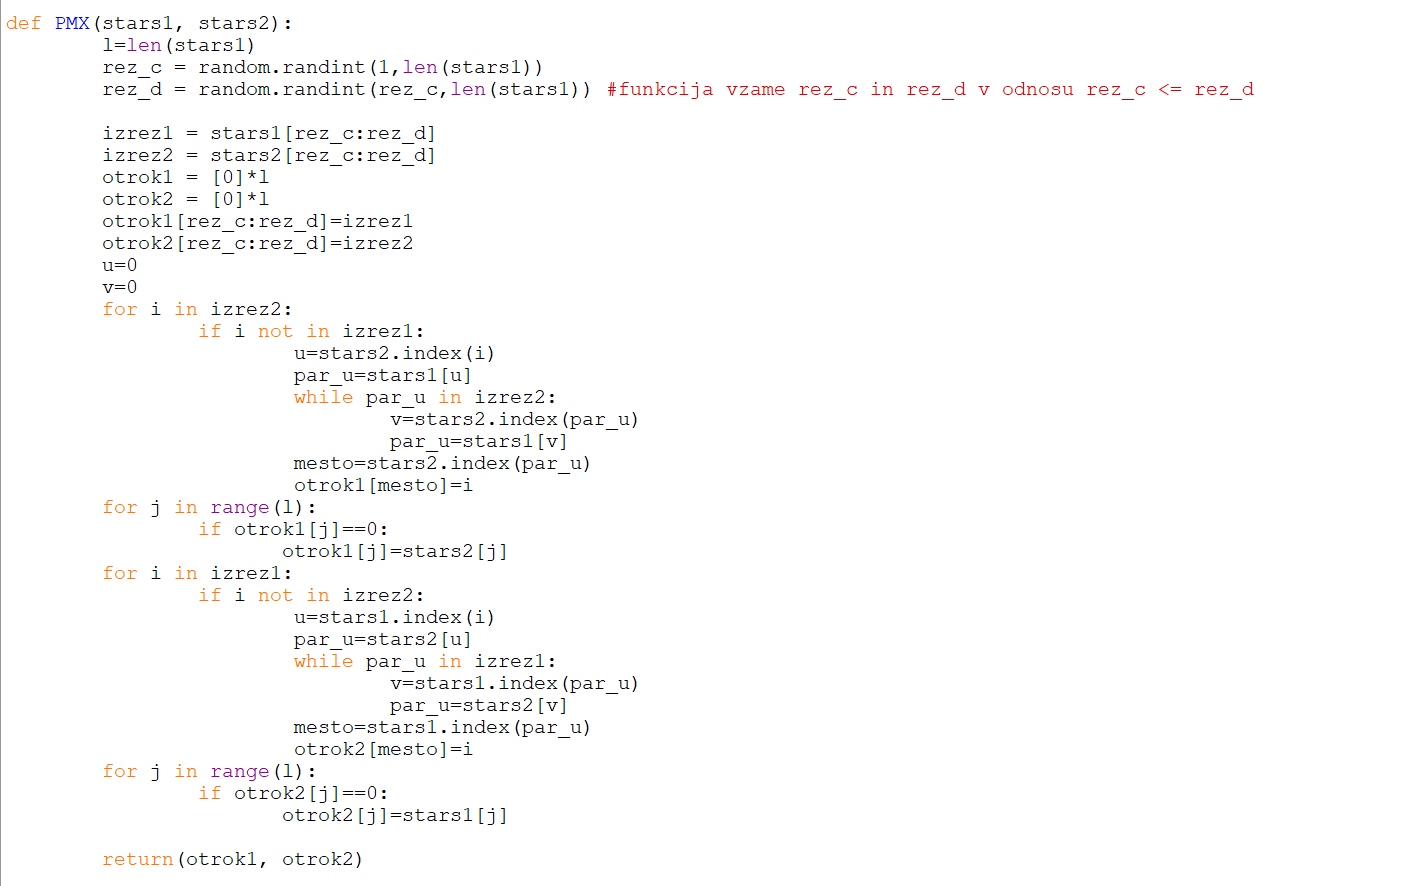
\includegraphics[width=1\textwidth]{PMX}
\end{figure*}
\newpage
\subsubsection{Ciklično križanje ali cycle crossover}
\
\\
\\
Zadnji način križanja, ki smo ga uporabili je ciklično križanje ali CX. Tu naša funkcija sprejme dva starša, iz katerih naredi slovar. Pri tem prvi starš predstavlja ključ, drugi pa vrednost. Najprej poiščemo vse ciklje med staršema in jih shranimo v množico A. Prvega otroka tvorimo tako, da mu po vrsti dodamo vsak sodi cikel iz prvega stašra in vsak lihi cikel iz drugega starša. Pri drugem otroku ravnamo ravno obratno.  

\begin{figure*}[ht]
\centering
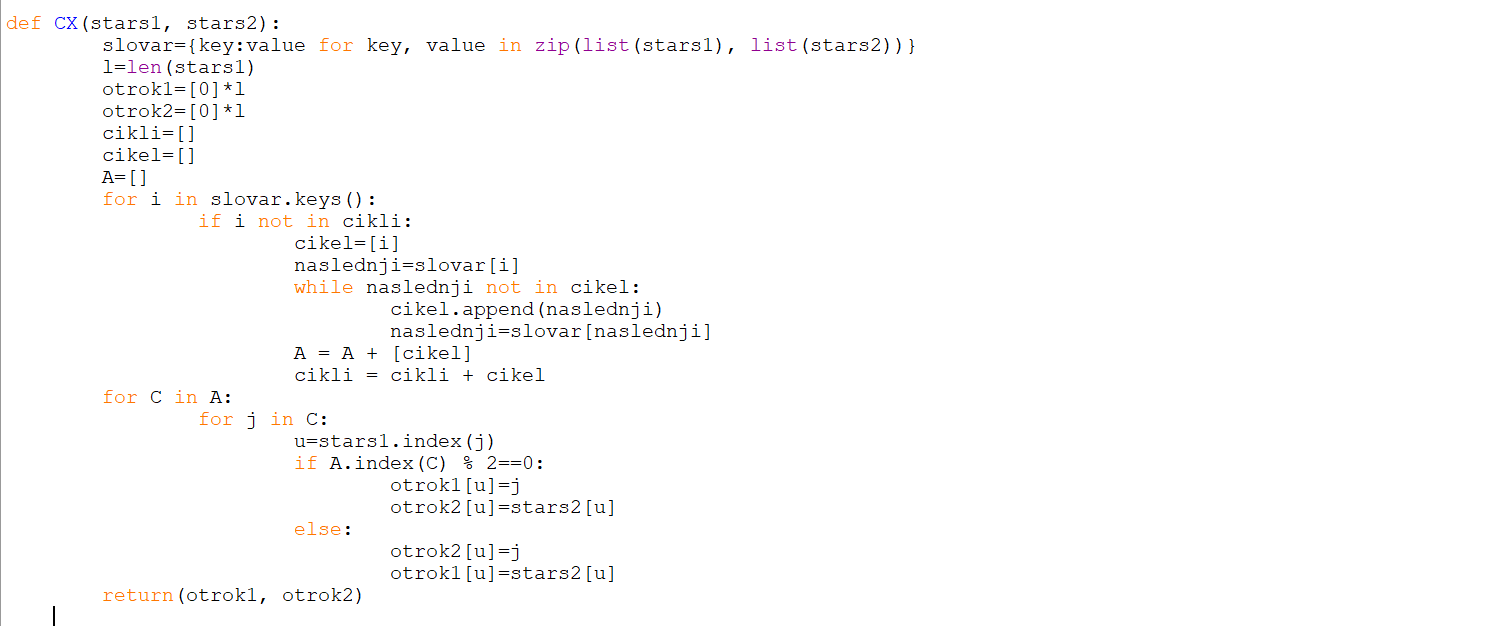
\includegraphics[width=1\textwidth]{CX}
\end{figure*}

\subsubsection{Naključno izbrano križanje}
\
\\
\\
Da bi bili rezultati še bolj zanimivi, smo napisali dodatno funkcijo \textit{nakljucno}, ki naključno izbere eno od križanj. 

\begin{figure*}[ht]
\centering
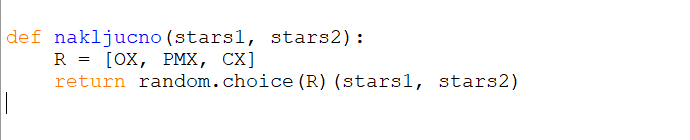
\includegraphics[width=1\textwidth]{nakljucno}
\end{figure*}

\newpage
\subsection{Mutacije}
\
\\
\\
S križanji smo dobili otroke, ki so neke nove poti ustvarjene iz dveh staršev. Da pa ohranjamo diverziteto v populaciji, je potrebno nekatere poti mutirati in sicer s \textit{SWAP mutacijo} (zamenjali bomo dve vozlišči v poti). Vsako vozlišče poti z neko verjetnostjo mutiramo, torej zamenjamo položaj mutiranega vozlišča z nekim naključnim vozliščem te poti. 
\begin{figure*}[ht]
\centering
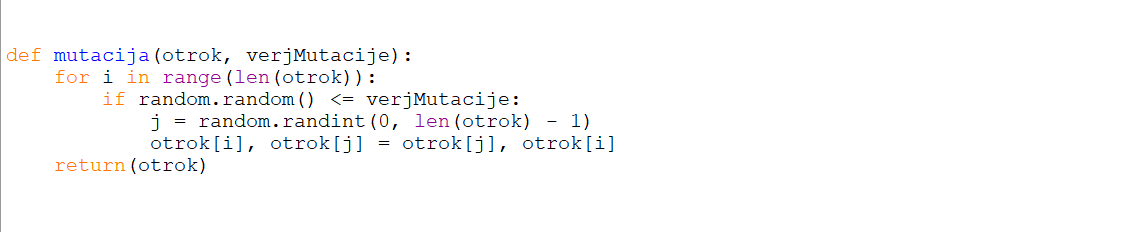
\includegraphics[width=1\textwidth]{mutacija}
\end{figure*}

Ker pa lahko potomce dobivamo na več načinov, se pravi z različnimi križanji smo za tvorbo potomcev napisali posebno funkcijo, ki sprejme več parametrov, med njimi tudi verjetnost mutacije in način križanja. 

\begin{figure*}[ht]
\centering
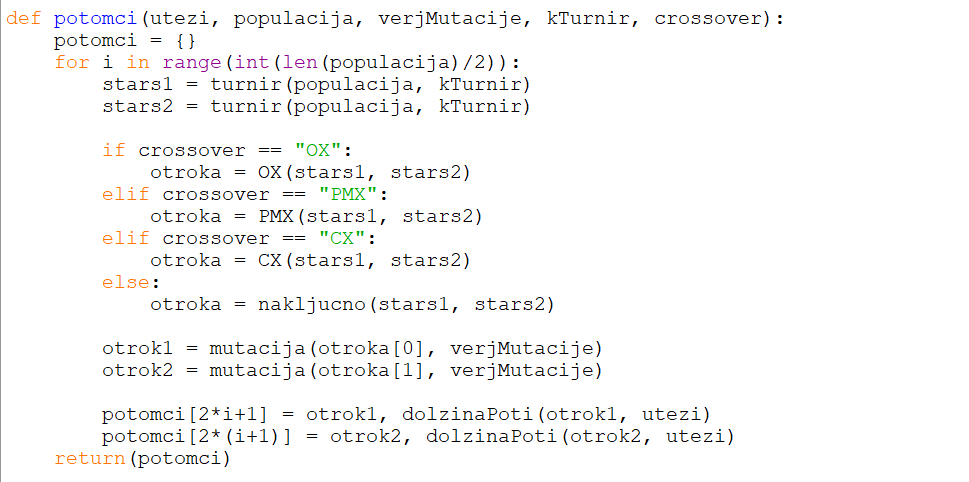
\includegraphics[width=1\textwidth]{potomci}
\end{figure*}
Cilj našega genetskega algoritma je najti najkrajšo pot, ki nam jo izračuna naslednja funkcija. 

\begin{figure*}[ht]
\centering
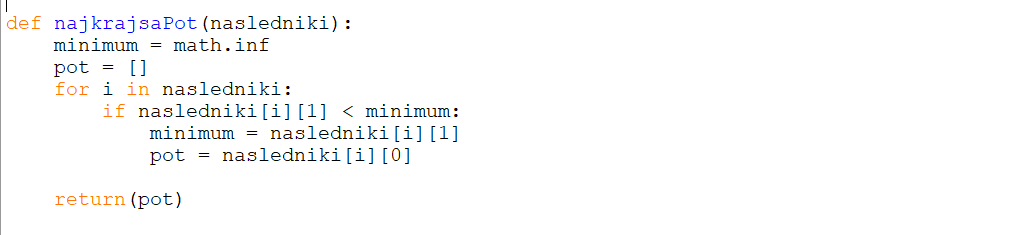
\includegraphics[width=1\textwidth]{najkrajsapot}
\end{figure*}

Po pridobitvi vseh potrebnih podatkov, lahko na tej točki poženemo naš genetski algoritem, ki nam izmed vseh poti iz dane generacije vrne najboljšo se pravi najkrajšo. 
\begin{figure*}[ht]
\centering
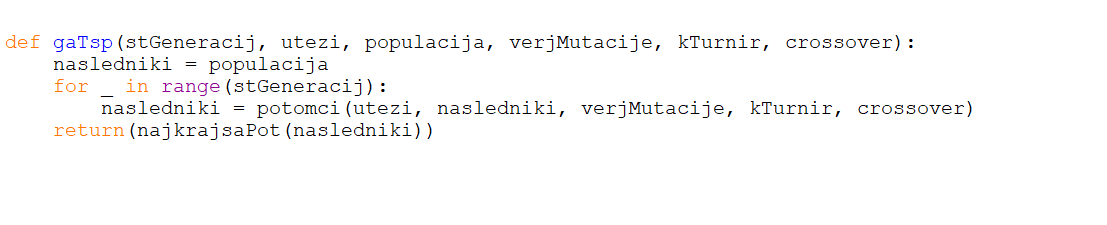
\includegraphics[width=1\textwidth]{gatsp}
\end{figure*}
\newpage

\subsection{Primeri in spreminjanje parametrov}
\
\\
\\
Za boljšo predstavo o delovanju našega algoritma smo na internetu poiskali nekaj že rešenih primerov in jih preizkusili tudi na našem genetskem algoritmu ter natu rezultate med sabo primerjali. Pri tem smo si za boljšo predstavo risali grafe s funkcijo \textit{narisi}  ter \textit{gaTspGraf}. 

\begin{figure*}[ht]
\centering
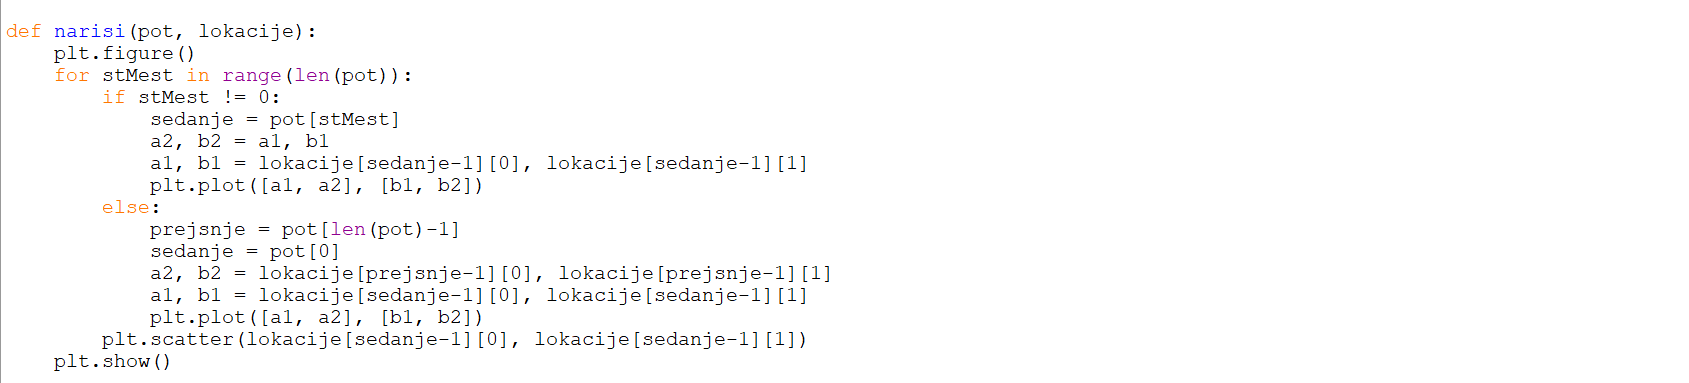
\includegraphics[width=1\textwidth]{narisi}
\end{figure*}

\begin{figure*}[ht]
\centering
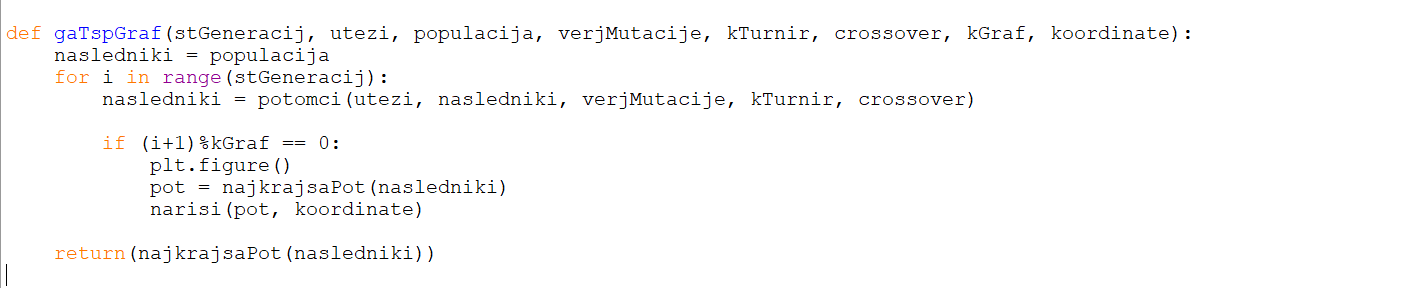
\includegraphics[width=1\textwidth]{gatspgraf}
\end{figure*}

Pri naših primerjavah nas je zanimala povprečna dolžina najkrajše poti, prav tako pa nam pomemben podatek predstavla tudi najkrajša pot v vseh ponovitvah. Funkcija \textit{povprecje} nam je pri danih ponovitvah genetskega algoritma izračunala povprečno dolžino njakrajše poti, ter hkrati tudi vrnila najkrajšo pot in njeno dolžino.

\begin{figure*}[ht]
\centering
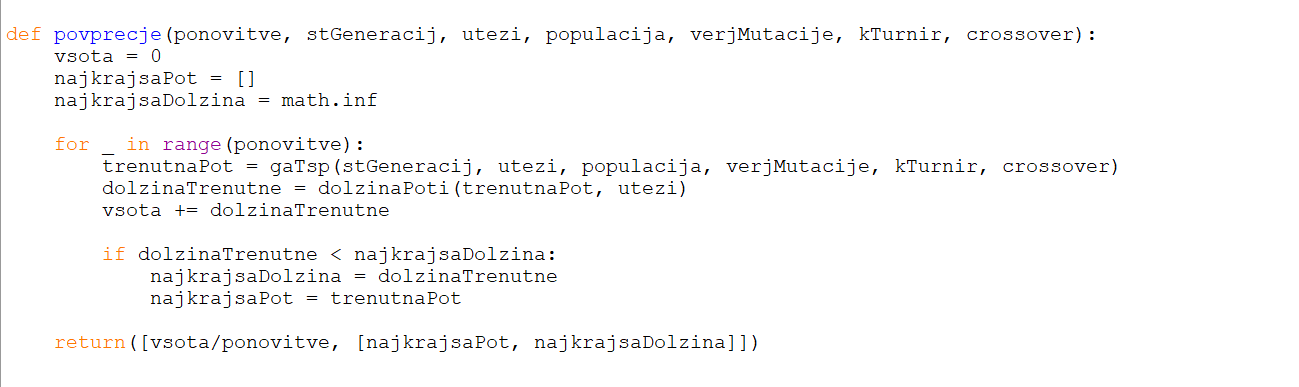
\includegraphics[width=1\textwidth]{povprecje}
\end{figure*}
\newpage

\section{Zaključek}

V naši analizi smo se osredotočili na tri primere, katerih podatke in približkih rešitve smo dobili na internetu. Nato smo rešitve za dane probleme, dobljene z našim genetskim algoritmom primerjali s tistimi z interneta. Omejili smo se na tri primere in sicer ulysses22, berlin52 in kroal100. Pri primeru berlin52 smo naredili veliko primerjav, da smo dobili občutek kateri parametri res vplivajo na kvaliteto rešitve. To smo potem primerjali in potrdili še na drugih dveh primerih. 
\\
\\
Tekom analize smo spreminjali sledeče parametre:
\begin{itemize}
\item križanje (CX, PMX in OX)
\item velikost populacije (20, 100)
\item število generacij (100, 1000)
\item verjetnost mutacije (0\%, 0.5\% in 4\%)

 \end{itemize}
Ohranjali pa smo število ponovitev 20 ter število kromosomov v turnirju nastavili na 5.
\\
\\
Pri primeru kroa100 je bila najbolj opazna sprememba ob večanju velikosti populacije. Dolžina najkrajše poti se je dokaj hitro bližala optimumu, kljub temu da so bile začetne vrednosti več kot dvakrat večje od optimalne vrednosti. 
Prav tako je bilo možno opaziti veliko spremembo ob povečanju števila generacij iz 100 na 1000, saj se je ob tem najkrajša pot dvakrat podaljšala.
\\
\\
Prav tako smo tudi pri primeru ulysses22 zasledili podobno gibanje rešitev, le da je bila tu konvergenca k optimumu precej hitrejša, saj sprememba števila generacij ne poveča vrednosti v tolikšni meri kot prej. Oba primera smo tu preizkušali le na urejenem križanju, med tem ko smo pri primeru berlin52 preizkusili čisto vse kombinacije. 
\\
\\
Začeli smo z cikličnim križanjem, katerega konvergenca je na začetku se pravi pri majhni populaciji, majhnem številu generacij in brez mutacije najbolj počasna od vseh treh križanj. Vrednosti naše rešitve so tudi trikratnik optimalne. Ko smo povečali velikost populacije se je rešitev rahlo izboljšala, vendar še vedno ne v meri, ki bi si jo želeli. Prav tako če smo povečali le število generacij. Ob povečanju obeh parametrov pa je bil približek rešitve že soliden. 
Nato smo povečali verjetnost mutacije iz 0 na 0.5 procenta in približek se je zelo izboljšal. Če smo ob tem še povečali populacijo in število generacij je bila vrednost rešitve najboljša do sedaj. 
Ko pa smo verjetnost mutacije povečali na 4 procente, je začela konvergenca padati. Ob povečanju števila generacij je bila ta že zelo počasna. 
S tem smo prišli do dejstva, da previsoka verjetnost mutacije negativno vpliva na rezultate. 
\\
\\
Pri delno mapiranem križanju je začetna vrednost malenkost boljša od tiste pri cikličnem križanju. Povečanje populacije v tem primeru porodi bistveno boljše rešitve kot pri enakem povečanju populacije v cikličnem križanju. 
Opazili smo tudi, da povečanje števila generacij tu ne vpliva bistveno na izboljšanje rešitev. Pri določenih primerih lahko konvergenco celo upočasni. 
Povečanje verjetnosti mutacije na pol procenta tudi tu bistveno izboljša rezultat. V kombinaciji z veliko populacijo je približek poti vedno bližje pravemu. 
Iz primerov vidimo, da večanje števila generacij najmanj pripomore k izboljšavi rešitve. 
Pri visoki verjetnosti mutacije vsi rezultati niso tako dobri, kar nam pove kako pomemben je ta dejavnik. Visoka verjetnost bolj negativno vpliva na PMX kot na CX vendar razlike niso velike. 
\\
\\
Najboljši začetni približek nam da urejeno križanje. Pri tem povečanje populacije izmerno vpliva na rezultat, saj rešitev postane dvakrat boljša. 
Med tem ko povečanje števila generacij spet pokvari rezultat. Z malo večjo verjetnostjo mutacije se rešitev približuje optimalni. Vendar pa pri visoki mutaciji (4\%) OX konvergira najpočasneje od vseh treh križanj. 
\\
\\
Opazimo, da se z večanjem velikosti populacije, pa tudi števila generacij rešitve izboljšujejo. Seveda pa ne smemo zanemariti dejstva, da z večanjem teh parametrov povečujemo tudi čas, ki ga algoritem potrebuje za izračun rešitve.  Glede na informacije o genetskih algoritmih smo zasledili, da naj bi se verjetnost mutacije gibala od 0.5 do 2 procenta. Verjetnost mutacije pri vrednosti 0.5\% nam v analizi dejansko da najbolše rešitve. Vidimo tudi, da je verjetnost mutacije (za vse tri metode) pri vrednosti 0.005 precej blizu optimalni, saj se že pri 0.01 in 0.02 dolžine poti (npr. pri OX) zopet večajo proti 12000. Se pravi lahko pri vseh primerih zasledimo, da preveliko povečanje verjetnosti mutacije negativno vpliva na približek rešitve. Mutacija, ki je seveda zelo pomembna za ohranjanje raznolikosti rešitev, pa ne sme zajeti prevelikega deleža populacije, saj se s tem izgubljajo naše že zgrajene rešitve. 
\\
\\
Če primerjamo izboljševanje rezultatov pri večanju populacije ali pa števila generacij opazimo, da na primer (pri OX) pri številu generacij 100 in velikosti populacije 50 dobimo rezultate okoli 12000, če desetkrat povečamo število generacij so najkrajše poti okoli 10000, pri desetkratni povečavi populacije pa okoli 8600. Torej je povečevanje populacije večjega pomena za konvergenco k optimalni rešitvi, kot povečava števila generacij.
\\
\\
 V splošnem je najhitrejša metoda z uporabo urejenega križanja ali OX. Na začetku so njeni rezultati sicer dokaj slabi, a jih lahko zelo hitro izboljšamo s povečanjem populacije in s tem povečamo hitrost konvergence. 

\newpage
\begin{thebibliography}{99}


\bibitem{wiki}
\emph{Genetic algorithm}, v: Wikipedia: The Free Encyclopedia, [ogled 13.~12.~201], dostopno na \url{https://en.wikipedia.org/wiki/Genetic_algorithm}.

\bibitem{splet}
N.~Kumar, Karambir in R.~Kumar, \emph{A Comarative Analysis of PMX, CX and OX Crossover operators for solving Travelling Salesman Problem}, [ogled 13.~12.~2018], dostopno na \url{http://www.mnkjournals.com/ijlrst_files/Download/Vol%201%20Issue%202/303-%20Naveen.pdf}.


\bibitem{primeri}
 \emph{ The TSPLIB Symmetric Traveling Salesman Problem Instances}, [ogled 28.~12.~2018], dostopno na \url{http://elib.zib.de/pub/mp-testdata/tsp/tsplib/tsp/index.html?fbclid=IwAR2VkUJ80JoqQbLKAyGlriphhbhYjwmE7f_gH1P5K6a0asRisrHoW_zKr48}




\end{thebibliography}{99}

\end{document}